\documentclass[conference]{IEEEtran}
\IEEEoverridecommandlockouts

\usepackage{cite}
\usepackage{amsmath,amssymb,amsfonts}
\usepackage{algorithmic}
\usepackage{graphicx}
\usepackage{textcomp}
\usepackage{xcolor}
\usepackage{booktabs}
\usepackage{multirow}
\usepackage{url}
\usepackage{listings}
\usepackage{float}

\lstset{
  basicstyle=\ttfamily\footnotesize,
  breaklines=true,
  frame=single,
  language=Verilog
}

\def\BibTeX{{\rm B\kern-.05em{\sc i\kern-.025em b}\kern-.08em
    T\kern-.1667em\lower.7ex\hbox{E}\kern-.125emX}}
\begin{document}

\title{Design and FPGA Implementation of a 5-Stage Pipelined RISC-V Processor with Software-Managed Sv32 TLB and Performance Analysis}

\author{\IEEEauthorblockN{Ved Patel}
\IEEEauthorblockA{\textit{Roll No: B24503} \\
\textit{SCEE --- School of Computing and Electrical Engineering} \\
\textit{Course Project --- VL326: Fundamentals of Processor Architecture and SoC Design}\\
Zybo Z7-10 (xc7z010clg400-1) \\
}
}

\maketitle

\begin{abstract}
This paper presents the design, verification, and FPGA deployment of a 5-stage in-order pipelined processor implementing the RISC-V RV32I base integer instruction set with Zicsr extension, augmented with a software-managed 4-entry fully-associative Translation Lookaside Buffer (TLB) using Sv32-style addressing and FIFO replacement. The processor features full data forwarding, load-use hazard detection, and a complete trap handling infrastructure supporting page fault exceptions with instruction replay. Empirical performance analysis across four test configurations with varying working-set sizes (1--16 pages) demonstrates a dramatic TLB capacity cliff: address-translation overhead rises from 39--42\% (cold-start misses only) to 87--88\% of total execution time under thrashing conditions, representing an 8$\times$ slowdown relative to an equivalent base CPU without virtual memory. Note that conventional CPI is \textit{not} a meaningful metric in this trap-replay architecture, since each TLB miss inflates both the cycle and instruction counts. The design is synthesized and deployed on a Digilent Zybo Z7-10 FPGA at 62.5~MHz, with performance data captured via Xilinx Integrated Logic Analyzer (ILA).
\end{abstract}

\begin{IEEEkeywords}
RISC-V, pipelined processor, TLB, virtual memory, Sv32, FPGA, page fault, FIFO replacement, ILA, performance analysis
\end{IEEEkeywords}

\section{Introduction}

Virtual memory is a foundational abstraction in modern computer systems, enabling process isolation, flexible memory management, and the illusion of a large, contiguous address space. The Translation Lookaside Buffer (TLB) is a critical performance component that caches recent virtual-to-physical address translations to avoid costly page table walks on every memory access.

This project investigates the following research question: \textit{What is the effective address-translation overhead as a fraction of total execution time when TLB coverage is exceeded?}

To answer this, we designed and implemented a complete RV32I pipelined processor with:
\begin{itemize}
    \item A 5-stage in-order pipeline (IF, ID, EX, MEM, WB) with full data forwarding and load-use hazard stalling
    \item Zicsr extension for Control and Status Register operations
    \item A 4-entry fully-associative TLB with FIFO replacement policy
    \item A software-managed page fault handler implementing 2-level Sv32 page table walks
    \item Performance counters for cycles, instructions, stalls, and TLB statistics
\end{itemize}

\textbf{Design scope.} This implementation makes three deliberate pedagogical simplifications relative to the full RISC-V Sv32 specification: (1)~only data memory accesses are translated---there is no instruction-side TLB; (2)~R/W/X/U permission bits from page table entries are not stored or enforced; and (3)~SATP is used purely as a base address register without MODE or ASID fields. These choices reduce hardware complexity while preserving the phenomena under study (TLB capacity effects and software page-walk overhead). They are explicitly documented as limitations in Section~\ref{sec:limitations}.

The design targets the Digilent Zybo Z7-10 FPGA board (Xilinx Zynq-7010) and uses Vivado 2025.2 for synthesis, implementation, and debugging via the Xilinx Integrated Logic Analyzer (ILA).

\section{Architecture Overview}

\subsection{Pipeline Design}

The processor implements a classic 5-stage in-order pipeline:

\begin{enumerate}
    \item \textbf{Instruction Fetch (IF)}: Priority-based PC mux supporting trap, MRET, branch, stall, and sequential paths. Fetches instructions from 16~KB BRAM.
    \item \textbf{Instruction Decode (ID)}: Decodes all 40 RV32I instructions plus 6 Zicsr instructions (CSRRW/RS/RC and immediate variants), ECALL, EBREAK, and MRET. Generates immediate values for all 5 formats (I/S/B/U/J).
    \item \textbf{Execute (EX)}: ALU operations (11 operations including PASS for LUI), branch resolution, misalignment detection, trap detection (6 cause codes), and CSR data computation.
    \item \textbf{Memory (MEM)}: TLB-based address translation, store data alignment with byte-enable masks, load data formatting (sign/zero extension for LB/LH/LW/LBU/LHU), and page fault generation.
    \item \textbf{Writeback (WB)}: 4-way result mux selecting from ALU, memory load, PC+4 (JAL/JALR), or CSR read data.
\end{enumerate}

\subsection{Data Hazard Management}

The processor implements two-level data forwarding:
\begin{itemize}
    \item \textbf{EX$\rightarrow$EX forwarding}: Bypasses results from the EX/MEM register to the current EX stage (excludes load instructions).
    \item \textbf{MEM$\rightarrow$EX forwarding}: Bypasses results from the MEM/WB register, including load data.
\end{itemize}

Load-use hazards are detected by the hazard unit, which inserts a 1-cycle pipeline bubble when an instruction in ID depends on a load currently in EX.

\subsection{Key Design Parameters}

Table~\ref{tab:params} summarizes the processor's design parameters.

\begin{table}[htbp]
\caption{Processor Design Parameters}
\begin{center}
\begin{tabular}{|l|l|}
\hline
\textbf{Parameter} & \textbf{Value} \\
\hline
ISA & RV32I + Zicsr \\
Pipeline depth & 5 stages \\
Data forwarding & EX$\rightarrow$EX and MEM$\rightarrow$EX \\
Branch resolution & EX stage (2-cycle penalty) \\
Branch prediction & Static not-taken \\
TLB & 4-entry, fully-associative, FIFO \\
Page size & 4~KB (12-bit offset) \\
Instruction memory & 16~KB BRAM \\
Data memory & 16~KB BRAM \\
Register file & 32 $\times$ 32-bit \\
Target FPGA & xc7z010clg400-1 (Zybo Z7-10) \\
CPU clock & 62.5~MHz (divided from 125~MHz) \\
\hline
\end{tabular}
\label{tab:params}
\end{center}
\end{table}

\section{CSR Infrastructure}

The processor implements 10 CSR registers essential for trap handling and TLB management:

\begin{itemize}
    \item \textbf{Standard M-mode CSRs}: MSTATUS (0x300), MTVEC (0x305), MSCRATCH (0x340), MEPC (0x341), MCAUSE (0x342), MTVAL (0x343), SATP (0x180)
    \item \textbf{Custom TLB CSRs}: TLB\_VPN (0xFC0), TLB\_PPN (0xFC1), TLB\_CMD (0xFC2)
\end{itemize}

CSR reads are combinational in the EX stage; writes are sequential in the MEM stage. Trap entry has priority over normal CSR writes, ensuring atomic save of MEPC, MCAUSE, and MTVAL.

The three custom CSRs provide a software interface for TLB management: the trap handler stages a VPN and PPN, then writes TLB\_CMD=1 to commit the entry or TLB\_CMD=2 to flush all entries.

\section{TLB Design and Virtual Memory}

\subsection{TLB Structure}

The TLB is a 4-entry fully-associative cache. Each entry stores only three fields: a valid bit, a 20-bit Virtual Page Number (VPN), and a 22-bit Physical Page Number (PPN)---totaling 43 bits per entry. Lookup is combinational; all four entries are compared in parallel against the requested VPN.

\textbf{Note on permission bits}: Unlike a full Sv32 TLB, our implementation does \textit{not} store or enforce R/W/X/U permission bits from the page table entries. All valid TLB hits allow both read and write access. This is a deliberate simplification---permission fault checking (RISC-V cause codes 5 and 7) is deferred to a future enhancement.

\subsection{FIFO Replacement Policy}

New entries are written at the position indicated by a 2-bit \texttt{next\_write\_index} counter, which increments on each write and wraps around ($0 \rightarrow 1 \rightarrow 2 \rightarrow 3 \rightarrow 0$). This provides deterministic, hardware-simple replacement.

\textbf{Justification}: FIFO was chosen over LRU for three reasons: (1) \textit{hardware cost}---FIFO requires only a 2-bit counter (2 flip-flops), while LRU for 4 entries needs $4 \times 2$-bit age counters plus priority logic ($\sim$10$\times$ more hardware); (2) \textit{benchmark equivalence}---for our sequential scan workloads, FIFO and LRU produce identical replacement decisions; and (3) \textit{research focus}---the TLB capacity cliff (the primary phenomenon under study) occurs identically under both policies when the working set exceeds TLB capacity.

\subsection{Translation Enable Conditions}

Address translation is active when \texttt{satp $\neq$ 0} AND \texttt{!handler\_mode}. The \texttt{handler\_mode} flag is set on trap entry and cleared on MRET, allowing the trap handler to access physical memory directly (identity-mapped) for page table walks.

\textbf{SATP simplification}: In the standard RISC-V Sv32 specification, SATP contains a MODE field (bit 31), an ASID field, and a 22-bit PPN. Our implementation uses SATP purely as a 32-bit base address register pointing to the root page table. Translation is enabled whenever SATP $\neq$ 0. There is no MODE bit, ASID, or privilege-mode gating. This is valid because the processor operates exclusively in M-mode.

\subsection{Page Fault Flow}

On a TLB miss:
\begin{enumerate}
    \item MEM stage detects miss, generates trap (cause 13 for loads, 15 for stores)
    \item Pipeline flushes; MEPC, MCAUSE, MTVAL saved to CSRs
    \item PC redirects to MTVEC (trap handler entry point)
    \item Software handler reads MTVAL, walks the 2-level Sv32 page table in data memory
    \item Handler writes TLB entry via custom CSRs (TLB\_VPN, TLB\_PPN, TLB\_CMD)
    \item MRET returns to MEPC, replaying the faulting instruction
    \item Replayed instruction hits in TLB and completes normally
\end{enumerate}

The measured miss penalty is 46 cycles per fault, comprising pipeline flush (4 cycles), handler execution (36 instructions + 2 load-use stalls), MRET pipeline flush (4 cycles), and instruction replay.

\section{FPGA Implementation}

\subsection{System Architecture}

The FPGA top module (\texttt{fpga\_top}) instantiates a clock divider (125~MHz $\rightarrow$ 62.5~MHz) and the \texttt{microprocessor} module. The clock divider ensures timing closure on the xc7z010's fabric.

\subsection{Debug Infrastructure: ILA}

Performance data is captured via a Xilinx Integrated Logic Analyzer (ILA) debug core with 15 probes (269 bits total) and 1024-sample depth. This replaced an earlier UART-based reporting interface (\texttt{perf\_reporter} + \texttt{uart\_tx}), eliminating the need for external USB-UART cables.

The ILA captures all six performance counters (total cycles, stall cycles, instruction count, TLB accesses/hits/misses), the program counter, data memory address, pipeline valid bits, real-time TLB signals, and CPU status. The primary trigger is the rising edge of \texttt{cpu\_halted}, with the trigger position set to mid-buffer (512 samples pre/post) for comprehensive capture around the halt event.

The ILA consumes approximately 8 BRAMs (6.7\% of the Z7-10's 120 BRAMs), a modest resource cost that enables powerful non-intrusive debugging.

\subsection{LED Status Indicators}

Four LEDs provide real-time status: LED0 indicates CPU halt, LED1 signals trap events, LED2 pulses on TLB misses, and LED3 provides a heartbeat from the cycle counter.

\section{Verification}

The design was verified through four progressively complex testbenches, each targeting a specific verification phase.

\subsection{Phase 0: RV32I Pipeline Regression}

A 49-instruction test program exercises all RV32I instructions through the pipeline, including forwarding paths, load-use stalls, and branch flushes. All 32 registers were verified against expected values.

\textbf{Results}: 53 cycles, 39 retired instructions, 1 stall cycle, CPI = 1.36. \textbf{32/32 register tests passed.}

\subsection{Phase 1: CSR Infrastructure}

A 70-instruction test verifies CSRRW/CSRRS/CSRRC/CSRRWI operations and the complete ECALL $\rightarrow$ MTVEC $\rightarrow$ handler $\rightarrow$ MRET $\rightarrow$ continue flow.

\textbf{Results}: \textbf{9/9 tests passed.}

\subsection{Phase 2--3: VM/TLB Full-Flow}

An 85-instruction test exercises end-to-end virtual memory: TLB lookups, page fault traps, 2-level page table walks, TLB refill, TLB flush (SFENCE), and instruction replay for both loads and stores.

\textbf{Results}: 16 TLB accesses, 9 hits, 7 misses (6 load faults + 1 store fault). \textbf{All 16/16 checks passed.}

\subsection{Phase 4--5: TLB Performance Benchmarks}

Four test configurations with varying working-set sizes characterize TLB performance. Each test uses the same benchmark program with different page counts (Table~\ref{tab:perf}).

\begin{table}[htbp]
\caption{TLB Performance Results (Simulation)}
\begin{center}
\begin{tabular}{|c|c|c|c|c|c|}
\hline
\textbf{Test} & \textbf{Pages} & \textbf{Accesses} & \textbf{Hits} & \textbf{Misses} & \textbf{Hit Rate} \\
\hline
T1 & 1 & 11 & 10 & 1 & 90\% \\
T2 & 4 & 44 & 40 & 4 & 90\% \\
T3 & 8 & 160 & 80 & 80 & 50\% \\
T4 & 16 & 320 & 160 & 160 & 50\% \\
\hline
\end{tabular}
\label{tab:perf}
\end{center}
\end{table}

\subsection{FPGA Deployment}

The design was successfully synthesized, implemented, and deployed on the Zybo Z7-10 FPGA at 62.5~MHz. Performance data was captured via the ILA debug core in Vivado Hardware Manager. The ILA waveforms confirmed the expected counter values, validating the FPGA implementation against simulation results.
\section{Performance Analysis}

\subsection{Experimental Methodology}

Performance data was collected from \textbf{FPGA hardware} (Zybo Z7-10 at 62.5~MHz) using the Xilinx ILA debug core, which captures cycle-accurate counter values at CPU halt. The benchmark program (\texttt{t\_perf\_instr.mem}) is \textbf{identical} across all four tests---only the data memory initialization file changes (varying page counts), ensuring the only independent variable is working-set size. Each test was run by re-programming the bitstream. Results are deterministic: identical bitstreams produce identical counter values. The memory model uses single-cycle BRAM with no cache hierarchy.

\subsection{TLB Capacity Cliff}

The results reveal a dramatic performance cliff at the TLB capacity boundary (4 entries):

\begin{itemize}
    \item \textbf{T1/T2 ($\leq$4 pages)}: 90\% hit rate. Only cold-start misses occur.
    \item \textbf{T3/T4 ($>$4 pages)}: 50\% \textit{observed} hit rate, but the \textbf{logical miss rate is 100\%}. This observed 50\% is \textbf{misleading as a performance indicator}: it arises from instruction replay, where each miss triggers a handler that refills the TLB, then the faulting instruction re-executes and hits, producing $2N$ observed accesses from $N$ logical misses. All subsequent analysis uses the \textit{logical} miss rate.
\end{itemize}

\subsection{Miss Penalty Analysis}

The trap handler at PC \texttt{0x200--0x28C} performs a 2-level software page table walk in 36 instructions: context save (6), address parsing (5), L1 walk (5), L2 walk (6), TLB fill (4), context restore (6), and MRET (1). Including pipeline flush penalties (4~cycles entry + 4~cycles MRET) and 2 load-use stalls, the analytical per-miss cost is \textbf{46~cycles}.

Cross-validation via the T3$\leftrightarrow$T4 differential yields $(8215-4135)/(160-80) = 51$~cycles, slightly higher because it includes additional baseline loop iterations.

\subsection{Formal Definitions}

\textbf{Definition (Address-Translation Overhead).} The fraction of total execution time attributable to address translation:
\begin{equation}
    \text{Overhead} = \frac{C_{\text{vm}} - C_{\text{baseline}}}{C_{\text{vm}}} \times 100\%
\end{equation}
where $C_{\text{vm}}$ is the measured cycle count with translation enabled, and $C_{\text{baseline}}$ is the cycle count for the identical workload on a base CPU without translation. Normalization is by $C_{\text{vm}}$ (not $C_{\text{baseline}}$) because we measure what fraction of the \textit{actual} execution is overhead, not how much slower the system became.

The baseline was derived from \textbf{the original base RV32I CPU} (before TLB/CSR integration), running the identical loop structure (10 outer iterations $\times$ $N$ inner data accesses). Both CPUs share the same 5-stage pipeline, forwarding paths, and 2-cycle taken-branch penalty, ensuring the comparison isolates TLB overhead. The formula $C_{\text{baseline}} = 60N + 38$ was verified by pipeline trace analysis and cross-checked against the base CPU's performance counters.

\subsection{Results}

\begin{table}[htbp]
\caption{Complete Performance Results from FPGA ILA}
\begin{center}
\begin{tabular}{|c|c|c|c|c|c|c|c|}
\hline
\textbf{Test} & \textbf{Pg} & \textbf{Cycles} & \textbf{Instrs} & \textbf{Misses} & \textbf{CPI} & \textbf{Hit\%} & \textbf{Overhead\%} \\
\hline
T1 & 1 & 160 & 128 & 1 & 1.25 & 90.9 & 38.8 \\
T2 & 4 & 475 & 356 & 4 & 1.33 & 90.9 & 41.5 \\
T3 & 8 & 4,135 & 3,252 & 80 & 1.27 & 50.0 & 87.5 \\
T4 & 16 & 8,215 & 6,452 & 160 & 1.27 & 50.0 & 87.9 \\
\hline
\end{tabular}
\label{tab:results}
\end{center}
\end{table}

Instruction counts were verified analytically: $\text{total} = \text{main\_instrs} + (\text{misses} \times 36)$, matching all four ILA captures exactly. The CPI values (1.25--1.33) appear similar because the instruction counter includes handler instructions; the meaningful metric is overhead percentage.

\textbf{Memory model caveat}: These results assume \textbf{ideal single-cycle BRAM}. In a real system with DRAM, page table walk loads would incur cache miss latency (50--200 cycles), inflating miss penalty from 46 to 200--500+ cycles. The \textit{relative} overhead trend remains valid regardless of memory technology.

\begin{figure}[htbp]
\centerline{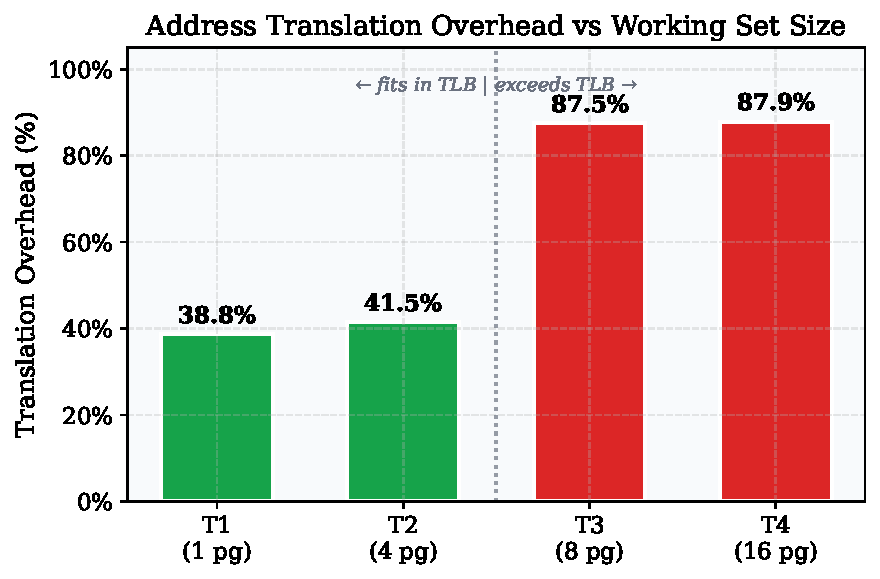
\includegraphics[width=\columnwidth]{figures/overhead_pct.pdf}}
\caption{Address translation overhead as a fraction of total execution time. The TLB capacity cliff is visible: overhead jumps from 39--42\% (fits in TLB) to 87--88\% (exceeds TLB).}
\label{fig:overhead}
\end{figure}

\begin{figure}[htbp]
\centerline{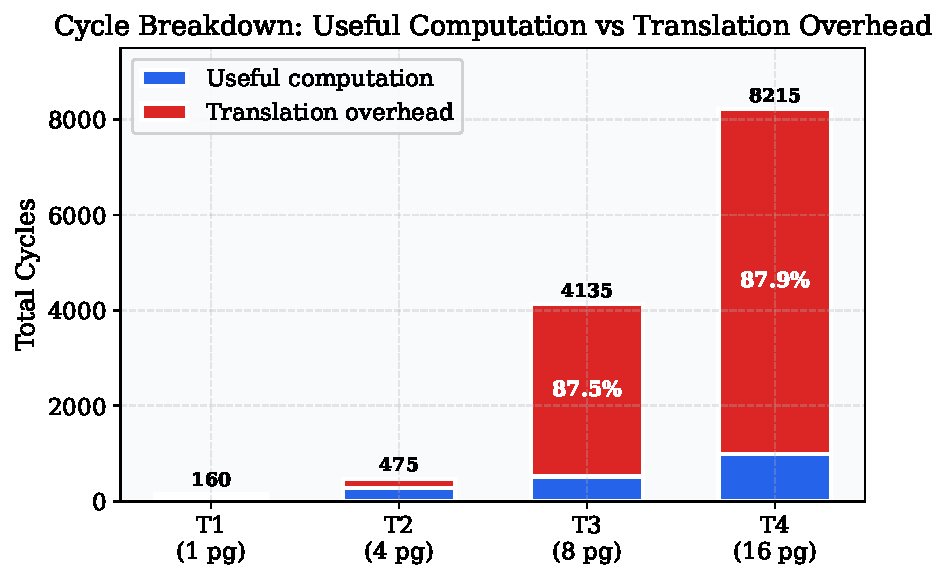
\includegraphics[width=\columnwidth]{figures/cycle_breakdown.pdf}}
\caption{Cycle breakdown showing useful computation (blue) vs translation overhead (red). Under thrashing (T3/T4), the processor spends nearly all cycles executing the trap handler.}
\label{fig:breakdown}
\end{figure}

\begin{figure}[htbp]
\centerline{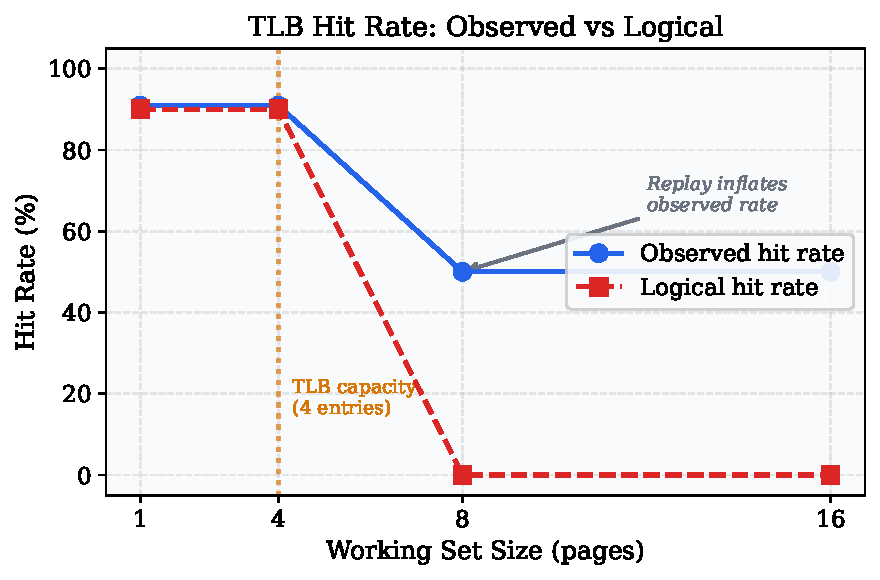
\includegraphics[width=\columnwidth]{figures/hit_rate.pdf}}
\caption{TLB hit rate: observed vs logical. The observed 50\% under thrashing is misleading---it arises from instruction replay. The logical miss rate is 100\%.}
\label{fig:hitrate}
\end{figure}

\begin{figure}[htbp]
\centerline{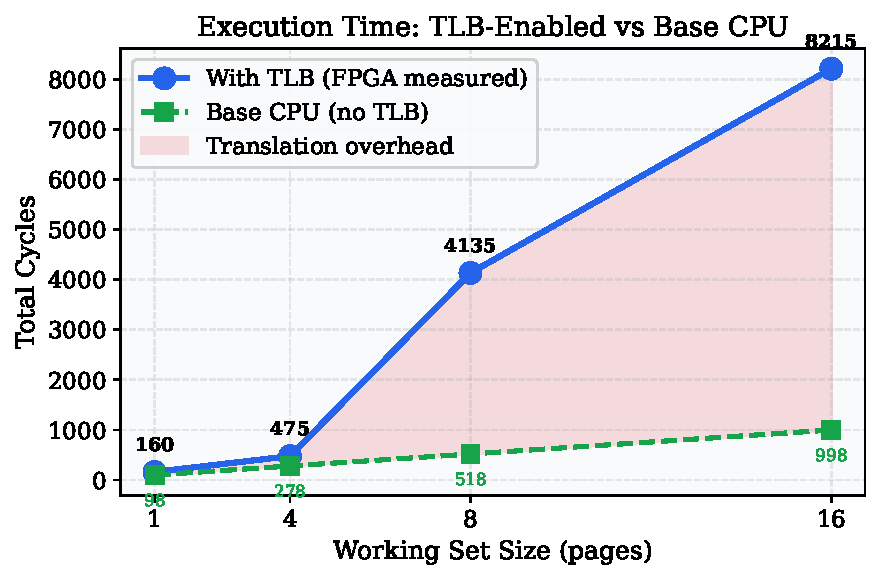
\includegraphics[width=\columnwidth]{figures/cycles_comparison.pdf}}
\caption{Total execution cycles with VM enabled (measured via FPGA ILA) vs base CPU without TLB. The shaded region represents the translation overhead. Both CPUs share identical pipeline and branch penalty.}
\label{fig:cycles}
\end{figure}

\begin{figure}[htbp]
\centerline{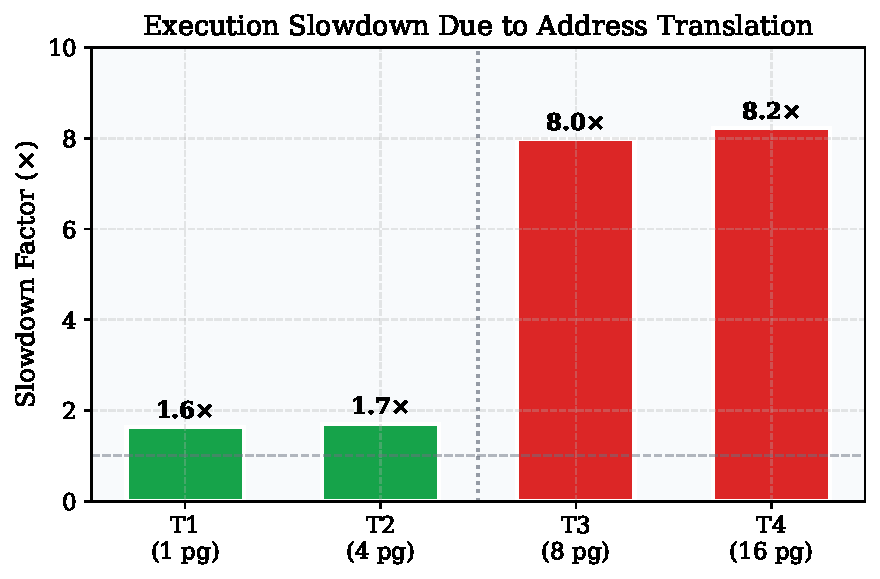
\includegraphics[width=\columnwidth]{figures/slowdown.pdf}}
\caption{Execution slowdown factor relative to the base CPU. Under thrashing (T3/T4), the TLB-enabled CPU is $\sim$8$\times$ slower.}
\label{fig:slowdown}
\end{figure}

\subsection{EMAT Analysis}

For theoretical completeness, the Effective Memory Access Time provides a standard metric:
\begin{equation}
    \text{EMAT} = h \times t_{\text{hit}} + (1-h) \times (t_{\text{hit}} + t_{\text{miss}})
\end{equation}
where $h$ is the \textit{logical} hit rate (not the observed rate inflated by replays), $t_{\text{hit}} = 1$~cycle, and $t_{\text{miss}} = 46$~cycles. For T1/T2 ($h=0.909$): $\text{EMAT} = 0.909 + 0.091 \times 47 = 5.2$~cycles. For T3/T4 ($h=0$, logical): $\text{EMAT} = 47$~cycles. Note that EMAT is a \textit{theoretical reference} assuming a simple cache-like model; the primary performance metric in this work is the directly measured overhead percentage, which captures the full system behavior including pipeline flushes and instruction replay.

\begin{figure}[htbp]
\centerline{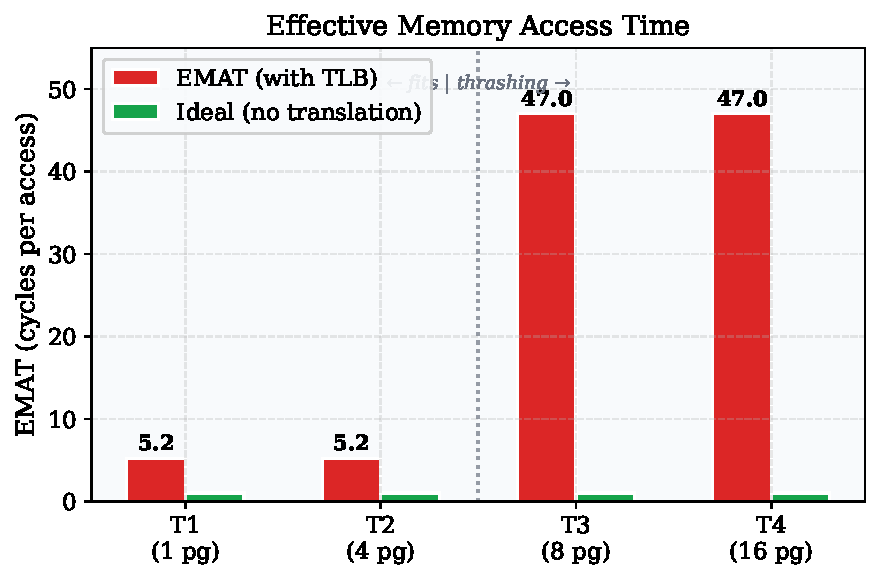
\includegraphics[width=\columnwidth]{figures/emat.pdf}}
\caption{Effective Memory Access Time: 5.2 cycles when fitting in TLB vs 47 cycles under thrashing (47$\times$ the ideal single-cycle access).}
\label{fig:emat}
\end{figure}

\begin{figure}[htbp]
\centerline{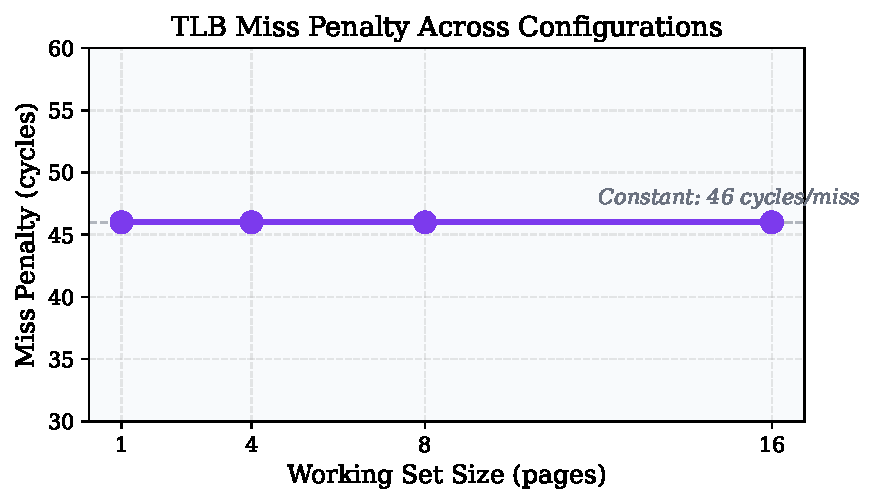
\includegraphics[width=\columnwidth]{figures/miss_penalty.pdf}}
\caption{TLB miss penalty remains constant at 46 cycles across all configurations, confirming deterministic handler execution independent of working-set size.}
\label{fig:misspenalty}
\end{figure}

\subsection{Answer to Research Question}

When the working set fits in the TLB, overhead is 38.8\% (T1) to 41.5\% (T2)---only cold-start misses, which would be amortized in longer programs. When TLB capacity is exceeded, overhead jumps to \textbf{87--88\%}: 87.5\% for 8~pages (2$\times$~TLB) and 87.9\% for 16~pages (4$\times$~TLB). The TLB-enabled CPU is $\sim$8$\times$ slower than the base CPU under thrashing. Each miss costs 46~cycles, and in the thrashing regime the processor spends nearly all its time in the trap handler. This confirms that TLB sizing relative to working-set size is the single most critical determinant of memory system performance in a software-managed TLB architecture.

\section{Design Evolution}

The architecture was developed in five phases:

\begin{enumerate}
    \item \textbf{Phase 0}: Base 5-stage pipelined RV32I processor with forwarding, hazard detection, and full ISA verification.
    \item \textbf{Phase 1}: CSR infrastructure (MSTATUS, MTVEC, MEPC, MCAUSE, MSCRATCH, SATP) and ECALL/MRET trap flow.
    \item \textbf{Phase 2--3}: 4-entry TLB with FIFO replacement, page fault handling, software trap handler, and handler\_mode for identity-mapped page table walks.
    \item \textbf{Phase 4}: FPGA deployment with clock divider, initially UART-based performance reporting (later replaced by ILA).
    \item \textbf{Phase 5}: Performance benchmarking with 4-test suite across varying working-set sizes.
\end{enumerate}

A significant infrastructure change was the replacement of the UART-based performance reporting system (\texttt{perf\_reporter.v} + \texttt{uart\_tx.v}, $\sim$286 lines) with a Xilinx ILA debug core. This simplified the design by removing the need for external USB-UART hardware and serial terminal software, while providing richer real-time debugging capabilities including pipeline state visibility and advanced triggering.

\section{Resource Utilization}

\begin{table}[htbp]
\caption{FPGA Resource Summary (Post-Place-and-Route)}
\begin{center}
\begin{tabular}{|l|c|c|c|}
\hline
\textbf{Resource} & \textbf{Used} & \textbf{Available} & \textbf{Util.} \\
\hline
Slice LUTs & 9,395 & 17,600 & 53.4\% \\
\quad LUT as Logic & 5,978 & 17,600 & 34.0\% \\
\quad LUT as Distributed RAM & 2,324 & 6,000 & 38.7\% \\
\quad LUT as Shift Register & 1,093 & 6,000 & 18.2\% \\
Slice Registers & 10,055 & 35,200 & 28.6\% \\
Slices & 3,797 & 4,400 & 86.3\% \\
BRAM (36K+18K) & 7.5 & 60 & 12.5\% \\
DSP48 & 0 & 80 & 0\% \\
Bonded IOBs & 6 & 100 & 6.0\% \\
\hline
\end{tabular}
\label{tab:resources}
\end{center}
\end{table}

\textbf{Timing closure}: All timing constraints were met. The worst negative slack (WNS) is $+1.206$~ns on the \texttt{cpu\_clk} domain (16~ns period, 62.5~MHz), indicating a critical path delay of 14.794~ns. Hold slack is $+0.015$~ns with zero failing endpoints across 42,509 total endpoints.

\textbf{Power}: Total on-chip power is 0.137~W (43~mW dynamic + 94~mW static). The ILA debug core consumes 25~mW (58\% of dynamic power); the CPU core itself uses only 11~mW. A production deployment without the ILA would reduce total power to approximately 0.112~W.

The design uses a modest fraction of the Z7-10's resources. The ILA debug core accounts for the majority of BRAM usage and register count increase from synthesis to implementation. Slice utilization at 86.3\% is the tightest resource constraint.

\section{Limitations and Future Work}
\label{sec:limitations}

\subsection{Current Limitations}

\begin{itemize}
    \item Static not-taken branch prediction incurs a 2-cycle penalty on every taken branch (IF/ID and ID/EX flushed).
    \item FIFO replacement does not exploit temporal locality; LRU would benefit workloads with hot/cold access patterns.
    \item Software page table walk (46 cycles measured) is significantly slower than a hardware walker ($\sim$2--5 cycles).
    \item No instruction TLB---only data memory accesses are translated.
    \item Single-cycle memory model does not reflect realistic cache miss latencies.
\end{itemize}

\subsection{Potential Enhancements}

\begin{itemize}
    \item LRU replacement policy (parameterized via \texttt{USE\_LRU} flag).
    \item Hardware page table walker for reduced miss penalty.
    \item Permission checking (R/W/X bits from PTE).
    \item Separate instruction TLB for fetch stage translation.
    \item Configurable TLB size (4/8/16 entries) for comparative analysis.
    \item Hot-cold access pattern benchmarks to demonstrate LRU advantage.
\end{itemize}

\section{Conclusion}

We have designed, verified, and deployed a complete RISC-V RV32I pipelined processor with software-managed Sv32-style virtual memory on the Zybo Z7-10 FPGA. The empirical performance analysis demonstrates that:

\begin{enumerate}
    \item The 4-entry FIFO TLB achieves 90.9\% observed hit rates when the working set fits within TLB capacity, with address-translation overhead of 39--42\% (cold-start misses that would amortize in longer programs).
    \item A sharp capacity cliff occurs when the working set exceeds 4 pages: the logical miss rate reaches 100\%, and address-translation overhead jumps to \textbf{87--88\%} of total execution time, representing an 8$\times$ slowdown versus the base CPU.
    \item Each TLB miss costs 46 cycles (pipeline flush, 36-instruction software handler, MRET, and instruction replay), as verified by consistent instruction count decomposition across all four FPGA captures.
    \item The ILA-based debug infrastructure provides efficient, non-intrusive performance data capture on FPGA hardware.
\end{enumerate}

The complete design comprises approximately 1,975 lines of synthesizable Verilog across 24 source modules, with 4 testbenches totaling $\sim$798 lines providing comprehensive verification coverage from individual instruction correctness to system-level virtual memory flows.

\section*{Acknowledgment}

This project was developed as part of the Computer Organization and Architecture course. The RISC-V ISA specification~\cite{b1} and the RISC-V Privileged Architecture specification~\cite{b2} provided the architectural foundation.

\begin{thebibliography}{00}
\bibitem{b1} A. Waterman and K. Asanovi\'{c}, Eds., ``The RISC-V Instruction Set Manual, Volume I: Unprivileged ISA,'' Document Version 20191213, RISC-V Foundation, Dec. 2019.
\bibitem{b2} A. Waterman and K. Asanovi\'{c}, Eds., ``The RISC-V Instruction Set Manual, Volume II: Privileged Architecture,'' Document Version 20211203, RISC-V Foundation, Dec. 2021.
\bibitem{b3} J. L. Hennessy and D. A. Patterson, \textit{Computer Architecture: A Quantitative Approach}, 6th ed. Cambridge, MA: Morgan Kaufmann, 2019.
\bibitem{b4} D. A. Patterson and J. L. Hennessy, \textit{Computer Organization and Design RISC-V Edition: The Hardware/Software Interface}, 2nd ed. Cambridge, MA: Morgan Kaufmann, 2021.
\bibitem{b5} Xilinx, ``Vivado Design Suite User Guide: Programming and Debugging,'' UG908, v2024.2, 2024.
\bibitem{b6} Digilent, ``Zybo Z7 Reference Manual,'' Rev. B, 2023. [Online]. Available: https://digilent.com/reference/programmable-logic/zybo-z7/reference-manual
\end{thebibliography}

\end{document}
